\documentclass[twoside,twocolumn]{ujarticle}
\usepackage{abstract}
\usepackage{url}
\usepackage[dvipdfmx]{graphicx}
\usepackage{amsmath,amssymb}
\usepackage{comment}

\newcommand{\bmath}[1]{\mbox{\boldmath $#1$}}

%%%%%%%%%% Parameters that should be customized %%%%%%%%%%
% Language (1 = Japanese, 2 = English)
\setlang{1}
% Bachelor or Master (1 = Bachelor, 2 = Master)
\setborm{1}
% Fiscal year
\setfy{2021}
% Group number
\setgnum{7}
% Presentation order
\setorder{6}
% Increase page number (optional)
%% \pplus{1}

% Title
\title{ANFISを用いたパターン識別における\\ノイズクラスタリング機構の導入}
% Author
\author{北森 頌規}
%%%%%%%%%% Parameters that should be customized (end) %%%%%%%%%%

\begin{document}
\maketitle
\small
\section{はじめに}
ANFIS~\cite{Jang1993}は,ファジィIf-Thenルールを利用することで高木-菅野ファジィ推論システム(TS-FIS)を導入した,説明可能なニューラルネットワークの一種である.
本論文では,ノイズファジィクラスタリングの概念に基づいた多クラス分類のためのロバストなANFISモデルを構築する手法を提案する.
分類器の学習に際して,教師クラスラベルにおけるノイズの存在を想定し,ノイズ個体による影響を排除することを考慮する.
\section{ノイズファジィクラスタリングに基づく\\ロバストなANFIS分類器}

%%%%%%%%%%%%%%%%%%%%%%%%ANFIS for classification%%%%%%%%%%%%%%%%%%%
多クラス($C$クラス)分類のためのANFISでは,
%図\ref{fig: ANFIS_architecture}に示すような,
5層のニューラルネットワークアーキテクチャによってファジィ推論を行う.
$n$個体の$m$次元入力と$C$次元出力のペア$((x_{i1}, \dots, x_{im})^\top, (y_{i1}, \dots, y_{iC})^\top)$があり,個体$i$がクラス$c$に所属するとき$y_{ic}=1$,それ以外を$y_{ic}=0$とするときに,$K$個のFuzzy If-Thenルールを用いて識別器を構築する.

\begin{comment}
\begin{figure}[hb]
\centering
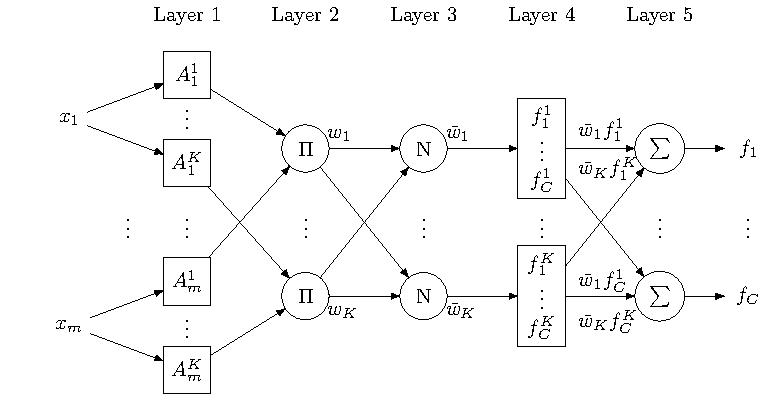
\includegraphics[width=.9\hsize]{anfis_architecture_classification.pdf}
\caption{\label{fig: ANFIS_architecture}多クラス分類のためのANFIS構造.}
\end{figure}
\end{comment}


%%%%%%%%%%%%%%%%%%%%%%%%noise fuzzy clustering%%%%%%%%%%%%%%%%%%%%%
主成分分析によるロバストな$k$-means法~\cite{Honda2010_IEEE-TFS}では,個体$i$の非ノイズ度とノイズ度を表すファジィメンバシップ$u_i$とその補数$1-u_i$をそれぞれ利用したロバストなPCAを$k$-means法に導入し,クラスター中心$\bmath{b}_c$をロバストに求めるための以下の目的関数の最小化を考える.
%
\begin{equation}
	J_{rkm} = \sum_{i=1}^n \left( (1-u_i)^\theta \gamma + u_i^\theta \sum_{k=1}^K \sum_{i \in G_k} || \bmath{x}_i - \bmath{b}_k||^2 \right)
\end{equation}
%
$\theta$がファジィ度を調整する重みであり,1に近づけるほどクリスプな分割に近づく.
$\gamma$は,各個体とノイズクラスタとの距離であり,全個体で共通の値を持つ.

%%%%%%%%%%%%%%%%%%%%%%%%noise robust ANFIS%%%%%%%%%%%%%%%%%%%%%%%%

実データの分析では,全個体に正しいラベルを付与することは困難であり,不正確なノイズラベルをもつ個体の影響を排除して分類器構築を行う必要がある.
そこで提案法では,多クラス分類のためのANFISにおいてノイズロバスト性を導入するアプローチとして,ノイズファジィクラスタリングの概念を導入し,以下の目的関数の最小化を考える.
%
\begin{equation}
	J_{ranfis} = \sum_{i=1}^n \left( (1-u_i)^\theta \gamma + u_i^\theta \sum_{c=1}^C (y_{ic} - \hat{y}_{ic})^2 \right)
\end{equation}
%
提案法におけるパラメータ最適化はLayer 5の回帰係数$\bmath{r}_c$の更新と勾配降下法によるLayer 1の前件部のファジィメンバシップ関数を定めるパラメータ$\phi_{kj}$の更新,および個体ごとの非ノイズ度$u_i$の更新を繰り返す.
%
\begin{equation}
	\bmath{r}_c = (W^\top U W)^{-1} W^\top U \tilde{\bmath{y}}_c
	\label{eq: LSE of coefficient vector}
\end{equation}
%
\begin{equation}
	\phi_{kj} \leftarrow \phi_{kj} - \tau \frac{\partial d_i}{\partial \phi_{kj}}
	\label{eq: premise parameters learning}
\end{equation}
%
\begin{equation}
	d_i = \sum_{c=1}^C (y_{ic} - \hat{y}_{ic})^2
\end{equation}
%
\begin{equation}
	u_{i} = \left( 1 + \left( \frac{d_i}{\gamma} \right)^{\frac{1}{\theta-1}} \right)^{-1}
	\label{eq: non-noise membership calculation}
\end{equation}
%
$\tilde{\bmath{y}}_c$は,$n$次元ベクトル$\tilde{\bmath{y}}_c=(y_{1c}, \dots, y_{nc})^\top$である.
$W$は,$n \times K$行列$W=\{ \bar{w}_{ik} \}$であり,$U$は,$i$番目の対角要素が$u_i^\theta$の$n \times n$対角行列である.
%

\section{数値実験}
%%%%%%%%%%%%%%%%%%%%%%%%実験方法%%%%%%%%%%%%%%%%%%%%%%%%

3種類のクラス($C=3$)からなる4次元($m=4$)の特徴量をもつIrisデータの中を,各クラス40個体ずつをランダムに抽出した120個体($n=120$)からなる訓練データと残りの30個体からなるテストデータに分割した.
また,提案法におけるノイズロバスト性は,以下のように調べた.
訓練データの一部のクラスラベルをランダムに10\%(12ノイズ個体),20\%(24ノイズ個体),30\%(36ノイズ個体),40\%(48ノイズ個体),50\%(60ノイズ個体)の5種類のノイズ比率を用いて変更し,そのノイズを含む訓練データを用いてANFISによる分類器を構築した.
ファジィ度と学習率,ノイズ感度は,それぞれ$\theta = 2$,$\tau = 0.00001$,$\gamma=1$と設定した.

%%%%%%%%%%%%%%%%%%%%%%%%実験結果%%%%%%%%%%%%%%%%%%%%%%%%

ノイズを含まない元の訓練データとノイズを含む訓練データに対して,従来法のANFIS分類器と提案法のANFIS分類器を構築した.
その分類性能を,訓練データでは表\ref{tab: classification ratios for training},テストデータでは表\ref{tab: classification ratios for test}に示す.

\begin{table}[!ht]
	\caption{訓練データに対する分類性能の比較}
	\label{tab: classification ratios for training}
	\centering
	\scalebox{.7}{
	{\tabcolsep = 2.5mm
	\begin{tabular}{c||c|c|c|c|c|c}\hline%\cline{3-11}
		ノイズ比率	& original& 10\% & 20\%	& 30\% 	& 40\% & 50\%    \\\hline\hline
		従来法	& 96.7\% & 86.7\% & 76.7\% & 70.8\% & 58.3\% & 48.3\%    \\\hline
		提案法 & 97.5\% & 86.7\% & 76.7\% & 67.5\% & 59.2\% & 51.7\%	 \\\hline
	\end{tabular}
	}}
\end{table}

\begin{table}[!ht]
	\caption{テストデータに対する分類性能の比較}
	\label{tab: classification ratios for test}
	\centering
	\scalebox{.7}{
	{\tabcolsep = 2.5mm
	\begin{tabular}{c||c|c|c|c|c|c}\hline%\cline{3-11}
		ノイズ比率	& original& 10\% & 20\%	& 30\% 	& 40\% & 50\%    \\\hline\hline
		従来法 & 100.0\% & 96.7\% & 96.7\% & 90.0\% & 86.7\% & 76.7\%    \\\hline
		提案法 & 100.0\% & 100.0\% & 96.7\% & 93.3\% & 90.0\% & 86.7\%	 \\\hline
	\end{tabular}
	}}
\end{table}

訓練データに対しては,ノイズ比率を考慮すると,分類性能が従来法と提案法どちらのモデルにおいてもほぼ完璧な分類性能($100\%-$ノイズ比率)を達成している.
一方,テストデータに対しては,提案法においてテストデータの汎化性能が従来法より向上していることがわかる.

\begin{comment}
\begin{figure}[htb]
\centering
\includegraphics[width=.8\hsize]{Final_mf_anfis_50.png}
\caption{従来法のメンバシップ関数 (ノイズ 50$\%$)}
\label{fig: membership of conventional ANFIS}
\end{figure}

\begin{figure}[htb]
\centering
\includegraphics[width=.8\hsize]{Final_mf_noise_50.png}
\caption{提案法のメンバシップ関数 (ノイズ 50$\%$)}
\label{fig: membership of proposed robust ANFIS}
\end{figure}

次に,従来法と提案法によるANFISから50\%のノイズラベルを含む訓練データで得られたファジィメンバシップ関数を比較する.
図\ref{fig: membership of conventional ANFIS}と図\ref{fig: membership of proposed robust ANFIS}では,4つの変量についてのルールごとのメンバシップ関数$\mu_{kj} (x_{j})$を比較している.
従来法では,データセットにノイズを含むとき属性$x_1$のルール2において,尖った形状の関数が得られた.
このような尖った形状は,いずれかのノイズ個体に対して過適合を起こしうる.
対して提案法では,訓練データにノイズラベルが含まれている場合でも変わらず,なめらかなメンバシップ関数を構築できている.

\end{comment}

\section{おわりに}
本論文では,ANFISによる分類器のノイズを含むクラスラベルに対するロバスト化を目的として,ノイズファジィクラスタリングの概念を導入する改良を提案し,数値実験により提案法の特性を示した.
今後は,クラス比が不均衡であったり,クラス境界の重複があるようなデータに対するノイズ感度を調査していく.
%なお,本研究の一部は,JSPS科研費 JP18K11474の助成に基づいて行われたものである.

\begin{thebibliography}{99}
	\bibitem{Jang1993}
	Jang, J.-S. R.: ANFIS: Adaptive-network-based fuzzy inference system, IEEE Trans. on Systems, Man and Cybernetics, 23-3, 665/685 (1993)

	\begin{comment}
	\bibitem{Takagi1985}
	Takagi, T., Sugeno, M.: Fuzzy identification of systems and its applications to modeling and control, IEEE Transactions on Systems, Man and Cybernetics, 15, 116/132 (1985)
\end{comment}


\bibitem{Honda2010_IEEE-TFS}
Honda, K., Notsu, A., Ichihashi, H.: Fuzzy PCA-guided robust $k$-means clustering, IEEE Trans. Fuzzy Systems, 18-1, 67/79 (2010)

\end{thebibliography}
\end{document}
